\textbf{COLUNI 2025 -- Questão 29}\par\medskip Observe a imagem abaixo que representa o ciclo de vida do mosquito \textit{Aedes aegypti}. Parte do desenvolvimento ocorre em depósitos de água naturais ou artificiais, onde, após a postura dos ovos, acontece a metamorfose; já a fase adulta do mosquito ocorre fora da água.

% COLUNI-AUTO-FIGURES-BEGIN
\begin{figure}[htbp]
\centering
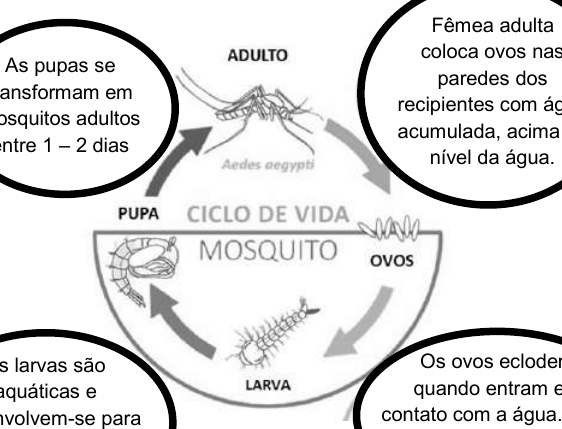
\includegraphics[width=0.8\linewidth]{static/simulados/coluni/figuras/2025/questao-29/figura-1.png}
\end{figure}
% COLUNI-AUTO-FIGURES-END
\noindent Disponível em: https://www.ecologiaesaude.com/post/ciclo-de-vida-do-aedes-aegypti. Acesso em: 03 set. 2024. Adaptado.

É CORRETO afirmar que a respiração de larvas e pupas, durante a metamorfose, e do mosquito adulto são, respectivamente, do tipo:
\begin{enumerate}
\item traqueal e cutânea.
\item branquial e traqueal.
\item pulmonar e branquial.
\item cutânea e pulmonar.
\end{enumerate}
